\section{Introduction}
\label{sec:intro}

A frontier model is expensive to train and cheap to query. That asymmetry makes \emph{distillation through the API} attractive: collect the model's answers to many well-chosen prompts and train a smaller model to imitate them \citep{hinton2015distilling,tramer2016stealing,orekondy2019knockoff}. Providers have long defended against this by flagging individual accounts whose queries look unusual \citep{juuti2019prada,zhang2021seat,sadeghzadeh2023hoda}. A capable attacker defeats that defence by spreading the campaign over many accounts, each of which then looks like an ordinary user. This is happening: in 2026 Anthropic reported distillation run through about 24{,}000 fraudulent accounts \citep{anthropic2026distillation} and campaigns that relayed real users' requests \citep{anthropic2026threat}; Google reported a campaign of more than 100{,}000 prompts \citep{google2026gtig}; and a joint U.S.\ government advisory described industrial-scale campaigns with automated failover to alternate access pathways \citep{cisa2026aa26251a}. Providers first try to \emph{link} such accounts through network, payment and device metadata, but a determined attacker can scrub those signals.

\paragraph{The question.} Suppose linkage has failed. The provider still sees every query from every account. \emph{Can it tell, from the queries alone, that a group of seemingly unrelated accounts is jointly extracting its model---and if so, when, at what false-alarm rate, and at what cost to the attacker?}

\paragraph{The short answer.} Query monitoring is worth running, but it is a filter, not a wall. What decides whether a campaign is visible is not a signature of extraction but \emph{benign coordination}: ordinary users also cluster on topics, follow trends, run evaluation scripts and paste templates. A campaign is visible only if it stands out more than the most distinctive group of ordinary users in the same week. We call this the \emph{benign-coordination barrier}; nearly every result below, positive or negative, follows from it.

\begin{figure}[t]
\centering
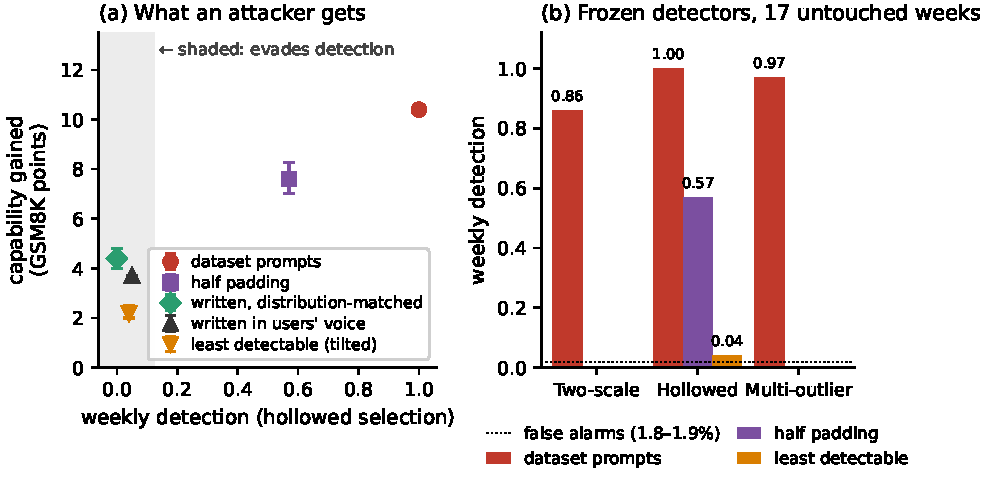
\includegraphics[width=\linewidth]{figs/glance.pdf}
\caption{The paper at a glance. (a) Capability a small student gains from 3{,}000 queries of each campaign type (GSM8K points; bars span two seeds) against how often hollowed selection, our most robust detector, catches the campaign each week (untouched weeks for the dataset, padded and least-detectable campaigns; development weeks for the two written ones). Every campaign in the shaded band evaded detection and kept at most 42\% of the dataset campaign's gain. (b) Three frozen detectors on 17 weeks that no design choice had touched; missing bars are zero. Only hollowed selection still catches campaigns padded with natural prompts; none catches the least-detectable campaign.}
\label{fig:glance}
\end{figure}

\paragraph{What this offers a provider.} We built and stress-tested a complete query-only monitor on real chat traffic \citep{zhao2024wildchat}, and distilled every campaign into a small student so that detection could be weighed against what the attacker gains (Figure~\ref{fig:glance}):
\begin{enumerate}[leftmargin=1.5em]
\item \textbf{Naive distributed extraction is catchable.} Dataset-like campaigns spread over many volume-matched accounts were caught in 86--100\% of weeks on data the monitor had never seen, at about 2\% false alarms; per-account monitors, tested on the development weeks, caught essentially none.
\item \textbf{The obvious evasion can be countered.} Padding every colluder account with natural prompts defeated our first detector. Judging accounts by whether they \emph{move together}, after discounting how topical each one is, still caught padded campaigns in 50--96\% of untouched weeks.
\item \textbf{Covertness was expensive in our testbed.} Every campaign that evaded every detector kept at most 42\% of what a detectable campaign transferred to a student that lacked the skill.
\item \textbf{The key quantity is measurable.} How coordinated a provider's benign traffic is decides what any monitor can see; it doubled between two periods of the same log, and we provide a script to measure it.
\end{enumerate}

\paragraph{What it cannot do.} Campaigns that relay real users' requests may have the same statistical law as real users, and then no query-only monitor can separate them. A campaign that ramps up slowly through the calibration weeks sharply cut the detection rate of every detector we built, two of them to near zero. At colluder shares of 2.5\% or below we found no detector that was both calibrated and powerful. And the monitor detects coordinated topic shift, not extraction: a customer benchmarking a model from ten accounts looks like a distiller.

\paragraph{How we kept ourselves honest.} Every experiment had predictions written into its notebook before it ran; of 184, 74 failed, and the full log is released with the code (\coderepo) together with the corrections we made along the way. Because later design choices were tuned on the same 24 development weeks, we froze the pipeline and evaluated it once on 17 later weeks from a different release of the log (Section~\ref{sec:holdout}); where the two disagree, the untouched weeks decide.

\paragraph{Contributions.} (i) A formal account of the benign-coordination barrier: law-matching campaigns are undetectable, a positive gap buys a detection \emph{time}, and the hardest campaign to detect is an exponential tilt of benign traffic whose capacity obeys a square-root law (Section~\ref{sec:theory}). (ii) A query-only monitor whose calibration survives weekly drift, with a hollowed variant that resists padding (Sections~\ref{sec:monitor} and~\ref{sec:results}). (iii) A capability--detectability frontier measured by distillation (Section~\ref{sec:frontier}). (iv) A frozen evaluation on untouched weeks with a second encoder (Section~\ref{sec:holdout}). (v) Code that reproduces every number, with each number mapped to the line that computes it and a complete record of predictions and corrections (Appendix~\ref{app:repro}).
